\newpage
\section{Laplace-Transformation}
	$$\boxed{F(s)=\int\limits_0^\infty f(t)e^{-st}dt} \qquad s=\sigma+j\omega$$\\
	- Definitionsbereich nur für kausale Systeme $t\geq 0$\\
	- Integrierbar über das Intervall $(0,\infty)$\\
	- Wachstum kleiner als der von eienr Exponentialfunktion\\ 
	- Gegen"uber $j\omega$ bei der Fourier-Transformation ist bei der
	Laplace-Transformation $s$ verallgemeinert zu $s=\sigma + j\omega$. Das
	bedeutet, dass die Fourier-Transformierte $F(j\omega)$ durch die
	Laplace-Transformation $F(s)$ ausgedr\"uckt werden kann.  	
  
 	\subsection{Eigenschaften}
  		\renewcommand{\arraystretch}{2}
		\begin{tabular}{|l|l|}
        	\hline
        	Linearität & 
 			$\alpha\cdot f(t) + \beta\cdot g(t) \laplace \alpha\cdot F(s) + \beta\cdot
 			G(s)$ \\
 			\hline
 			"Ahnlichkeit / Streckung &
 			$f(\alpha t) \laplace \frac{1}{\alpha}F \left (\frac{s}{\alpha} \right ) \quad 0
 			<\alpha \in\mathbb{R}$ \\
 			\hline
 			Faltung im Zeitbereich &
 			$f(t) \ast g(t) = \int\limits_{0}^{\infty} f(\tau)g(t-\tau)d\tau \laplace F(s)
 			\cdot G(s)$\\
 			\hline
 			Faltung im Frequenzbereich &
 			$f(t) \cdot g(t) \laplace \frac{1}{2\pi j}\int\limits_{c-j\infty}^{c+j\infty}
 			F(\xi) G(s-\xi)d\xi$ \\
 			\hline
 			Ableitung im Zeitbereich &
 			$\frac{\partial f(t)}{\partial t} \laplace sF(s)
 			-f(0+)$ \\
 			\hline
 			Ableitungen im Zeitbereich &
 			$\frac{\partial^n f(t)}{\partial t^n} \laplace s^nF(s)
 			-s^{n-1}f(0+)-s^{n-2}\frac{\partial f(0+)}{\partial t}-\ldots
 			-s^0\frac{\partial^{n-1} f(0+)}{\partial t^{n-1}}$ \\
 			\hline
 			Multiplikation mit $t$ &
 			$t\cdot f(t)  \laplace \frac{-\partial F(s)}{\partial s}$ \\
 			\hline
 			Ableitung im Frequenzbereich &
 			$(-t)^n f(t) \laplace  \frac{\partial^n F(s)}{\partial s^n}$ \\
 			\hline
 			Verschiebung im Zeitbereich &
 			$f(t\pm t_0) \laplace F(s)e^{\pm t_0 s}$ \\
 			\hline
 			Verschiebung im Frequenzbereich (Dämpfungssatz) &
 			$f(t)e^{\mp\alpha t} \laplace F(s\pm\alpha)$ \\
 			\hline
 			Integration &
 			$\int\limits_0^t f(\tau)d\tau \laplace \frac{F(s)}{s}$ \\
 			\hline
 			Anfangswert &
 			$\lim_{t\rightarrow 0} f(t) = \lim_{s\rightarrow \infty} sF(s),\text{~wenn
 			}  \lim_{t\rightarrow 0} f(t)\text{~existiert}.$ \\
 			\hline
 			Endwert &
 			$\lim_{t\rightarrow \infty} f(t) = \lim_{s\rightarrow 0} sF(s),\text{~wenn
 			}  \lim_{t\rightarrow \infty} f(t)\text{~existiert}.$ \\
 			\hline
       	\end{tabular}
		\renewcommand{\arraystretch}{\arraystretchOriginal}
	
	\subsection{Laplace-Tabelle}
	\begin{multicols}{2}
		\begin{center}
			\begin{tabular}{|lcc|}
				\hline
				$\sigma \left( t \right)$ & $\laplace$ & $\frac{1}{s}$ \\
				$\sigma \left( t \right) \cdot t$ & $\laplace$ & $\frac{1}{s^2}$\\
				$\sigma \left( t \right) \cdot t^2$ & $\laplace$ & $\frac{2}{s^3}$\\
				$\sigma \left( t \right) \cdot t^n$ & $\laplace$ & $\frac{n!}{s^{n+1}}$\\
				$\sigma \left( t \right) \cdot e^{\alpha t}$ & $\laplace$ &
				$\frac{1}{s-\alpha}$\\
				$\sigma \left( t \right) \cdot t \cdot e^{\alpha t}$ & $\laplace$ &
				$\frac{1}{( s - \alpha )^2}$\\
				\hline
			\end{tabular}
		\end{center}
	\columnbreak
		\begin{center}
			\begin{tabular}{|lcc|}
				\hline
				$\sigma \left( t \right)\cdot t^2 \cdot e^{\alpha t}$ &
				$\laplace$ & $\frac{2}{{( s - \alpha )}^3}$\\
				$\sigma \left( t \right)\cdot t^n \cdot e^{ \alpha t}$ &
				$\laplace$ & $\frac{n!}{(s-\alpha)^{n+1}}$\\
				$\sigma \left( t \right) \cdot \sin \left(\omega t \right)$ & $\laplace$ &
				$\frac{\omega}{s^2 + {\omega^2}}$\\
				$\sigma \left( t \right) \cdot \cos \left( \omega t \right)$ & $\laplace$ &
				$\frac{s}{ s^2 + \omega^2}$\\
				$\delta \left( t \right)$ & $\laplace$ & $1\left( s \right)$ \\
				$\delta \left( t - \alpha \right)$ & $\laplace$ & $e^{- \alpha s}$\\
				\hline
			\end{tabular}
		\end{center}
	\end{multicols}
		
	\subsection{Rücktransformation}
		\subsubsection{Vorgehen}
			\begin{tabular}{p{6cm}p{6cm}}
				1. Kürzen oder vereinfachen &
				3. Rücktransformation mittels Tabelle \\
				2. Partialbruchzerlegung falls nötig &
				4. $h(t)\hspace{0.2cm}\underline{nicht} < 0$ \\
			\end{tabular}
	
	\subsection{Lösung linearer Differentialgleichungen}

		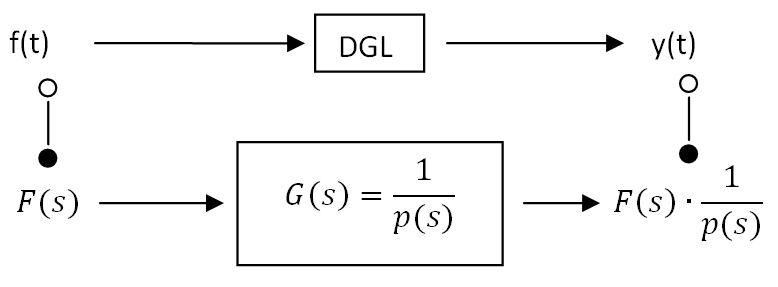
\includegraphics[width=10cm]{./bilder/diffgleichungen.png} \\
		\renewcommand{\arraystretch}{2}
		\begin{tabular}{| l | l |}
			\hline
				Übertragungsfunktion & $G(s) = \frac{1}{p(s)}$\\
				& $g(t) \laplace G(s)$ \\
			\hline
				Frequenzgang & $G(j\omega) = H(\omega)$ \\
			\hline
				Impulsantwort & $y_{\delta}(t) = g(t) \laplace G(s) = \frac{1}{p(s)}=Y_{\delta}(s)$\\
			\hline
				Sprungwantwort & $y_{\sigma}(t)=\int\limits_0^t g(u) du \laplace \frac{G(s)}{s} = \frac{1}{s \cdot p(s)} = Y_{\sigma}(s)$\\
			\hline
				Eigenschwingung & $\frac{h(s)}{p(s)}$ \\
			\hline
				äussere Erregung & $\frac{F(s)}{p(s)}$ \\
			\hline
				stationärer Zustand & = ungedämpfte Eigenschwingung\\
			\hline
		\end{tabular}
		\renewcommand{\arraystretch}{\arraystretchOriginal}\\
		
		\begin{minipage}[l]{16cm}
				\textbf{Beispiel:} $y'' + 8y' + 25y = \sigma{t} \cdot \sin(2t)$ mit $y(0) = 2, y'(0) = -1$\\
				
				$\sin(2t) \laplace \frac{2}{s^2+4}$ \\
				
				$\Rightarrow Y(s)(s^2+8s+25) = 2s+15+\frac{2}{s^2+4}$\\
				
				$\Leftrightarrow Y(s) = \frac{2s+15}{s^2+8s+25}+\frac{2}{(s^2+4)(s^2+8s+25)}=
				\underbrace{\frac{2s+15}{s^2+8s+25}}_\text{Eigenschwinung durch Anfangszustand} +
				\underbrace{\frac{As + B}{s^2+4}}_\text{stationärer Zustand} +
				\underbrace{\frac{Cs + D}{s^2+8s+25}}_\text{Eigenschwinung durch Einschalten}$
		\end{minipage}
		
		\subsubsection{Eigenschwingungen}
			Aus der Eigenschwingung können die Nullstellen des charakteristischen Polynom $p(s)$ 
			direkt abgelesen werden. \\
			\textbf{Beispiel:} \\
			$y(t) = \frac{1}{2} e^{-t} \sin(3t) - \frac{2}{3} e^{-2t} \cos(2t) = 
			\underbrace{\frac{1}{2} e^{\textcolor{red}{-t}} \frac{1}{2j}(e^{\textcolor{red}{3j}t}
			-e^{\textcolor{red}{-3j}t})}_{NS = EW = \textcolor{red}{-1 \pm 3j}} - 
			\underbrace{\frac{2}{3} e^{\textcolor{red}{-2}t} \frac{1}{2}(e^{\textcolor{red}{2j}t}
			+e^{\textcolor{red}{-2j}t})}_{NS = EW = \textcolor{red}{-2 \pm 2j}}$ \\\\
			Damit ist das char. Polynom $p(s) = (s-NS_1)(s-NS_2)\ldots(s-NS_n)$ \\\\
			Der stationäre Zustand ist $\lim\limits_{t\rightarrow\infty}y(t) = \frac{1}{p(0)}$ \\
			